\documentclass[10pt]{beamer}

\usepackage[utf8]{inputenc} 
\usepackage[T1]{fontenc}
\usepackage{lmodern}
\usepackage{graphicx}
\usepackage[english]{babel}
\usepackage{listings}
 %\usepackage{bbm}
\usepackage{color}
\usetheme{Warsaw}
\usepackage{lmodern}
\newtheorem{prop}{Proposition}
\usepackage{epsfig}
\setlength\abovecaptionskip{0.03ex}

 
\begin{document}
 
\title{\textbf{Backward Stochastic Differential Equation : Numerical Results}}
\author{ Majdi Rabia}
\maketitle

\AtBeginSection[]
{
  \begin{frame}
  \frametitle{Sommaire}
  \tableofcontents[currentsection,currentsubsection, hideothersubsections]
  \end{frame} 
}


\section{Introduction}

\begin{frame}
	\frametitle{Exmple of a Non-linear driver : bid-ask model}
	\[
	\left\{
	\begin{aligned}
	f(t,Y_t,Z_t) & =  -Z_t\theta  - rY + (R-r)(Y-\frac{Z_t}{\sigma})^-\\
	\theta &= \frac{\mu - r}{\sigma}\\
	\xi(X_T) & = (X_T - K_1) - 2(X_T - K_2)
	\end{aligned}
	\right.
	\]
	
	
\end{frame}


\section{Random Forest}

\subsection{Overview}

\begin{frame}{Overview}
	
	
	\centering
	\includegraphics[scale=0.2]{rf_general.png}
\end{frame}


\subsection{Most sensitive parameter}

\begin{frame}{Max leaf nodes}
	
	\centering
	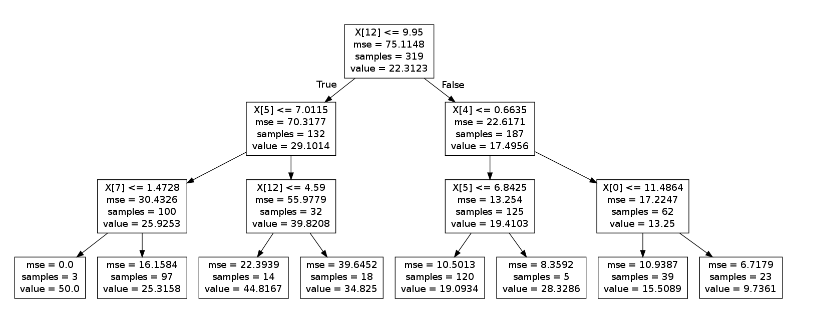
\includegraphics[scale=0.4]{max_leaf_nodes.png}
	
	This parameter helps avoid an overfitting by taking bigger values, but reaching a point, this will lead to some inaccuracies(cf following analysis on a specific example)
\end{frame}

\subsection{Other parameters}

\begin{frame}{Accuracy}
	\begin{itemize}
		\item \textbf{n\_estimators} : Represents the number of trees randomly generated. 
		We try to take the biggest value possible in our simulations, as the MSE decreases with this parameter. 
		\item \textbf{max\_features} : The number of features to consider when looking for the best split:
		\item \textbf{max\_depth} : The maximum depth of the tree
		\item \textbf{min\_samples\_split } : The minimum number of samples required to split an internal node
		\item \textbf{min\_samples\_leaf } : The minimum number of samples required to be at a leaf node
	\end{itemize}
	
\end{frame}

\begin{frame}{Performance}
	\begin{itemize}
		\item \textbf{n\_jobs} : The number of jobs to run in parallel for both fit and predict
		\item \textbf{warm\_start} : When set to True, reuse the solution of the previous call to fit and add more estimators to the ensemble, otherwise, just fit a whole new forest.
	\end{itemize}
	
\end{frame}

\subsection{Remarks}

\begin{frame}
	\begin{itemize}
		\item \textbf{Accuracy} : We focused especially on the maximum number of leafs allowed in the Random Forest simulation, which seemed to be the most sensitive parameter in one dimension. However, in higher dimension, results are not bad, but could be improved by constrain on other parameters. 
		\item \textbf{Performance} Warm\_start parameter could be helpful. From what I understand, it seems to keep in memory the last generated trees, and adding useful other estimators. This leads to better time performance, but I am going to analyse this on simple data to understand exactly how it works. 
		Indeed, it could be used for $\mathbb{E}[Y_{t+dt}|\mathcal{F}_t]$, as it is stable, but might be dangerous for $\mathbb{E}[Y_{t+dt}\Delta B_t|\mathcal{F}_t]$
	\end{itemize}
\end{frame}


\subsection{Max leaf nodes analysis (on European call example : expected 7.15)}

\begin{frame}{$N = 1000$}
	
	\centering
	\begin{figure}
		
	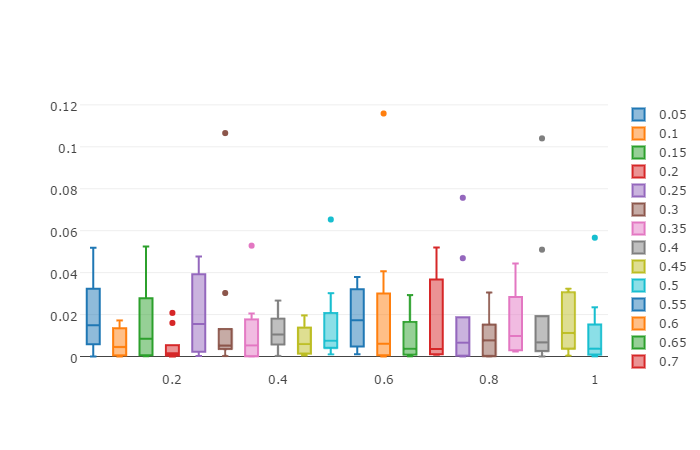
\includegraphics[scale=0.4]{max_leaf_1000.png}
	\caption{MSE against$\frac{RF\_max\_leaf\_nodes }{N}$  with N = 1000}
\end{figure}
\end{frame}


\begin{frame}{$N = 10000$}
	
	
	\begin{figure}
	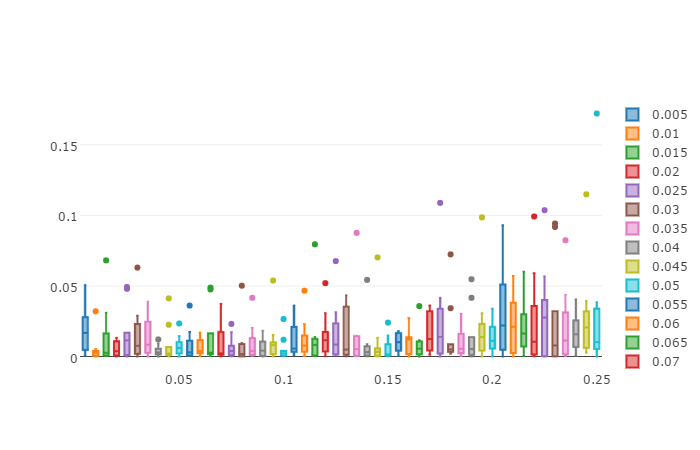
\includegraphics[scale=0.36]{max_leaf_10000.png}
	\caption{MSE against$\frac{RF\_max\_leaf\_nodes }{N}$  with N = 10000}
	\end{figure}
\end{frame}

\begin{frame}{$N = 10000$}
	
	\centering
	\begin{figure}
		
	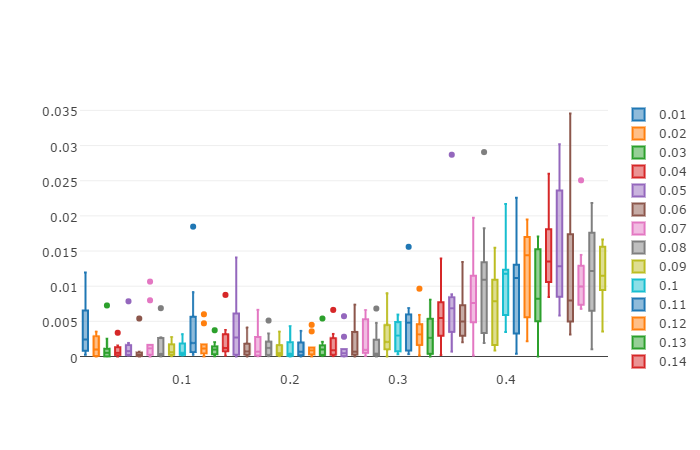
\includegraphics[scale=0.4]{max_leaf_100000.png}
	\caption{MSE against$\frac{RF\_max\_leaf\_nodes }{N}$  with N = 100000}
	
	\end{figure}
\end{frame}

\begin{frame}{Remarks}
	\begin{itemize}
		\item Getting a clear analysis from the previous three figures is not easy. It seems like there exists a stable region (with high variance) around 10 to 20\%. 
		\item We will take 10\% in the following simulations.
	\end{itemize}
\end{frame}

\subsection{Parameter fitting : min\_samples\_split and min\_samples\_leaf}

\begin{frame}
	
\end{frame}


\section{Applications}


\begin{frame}
	\frametitle{Overview}
	
	\centering
	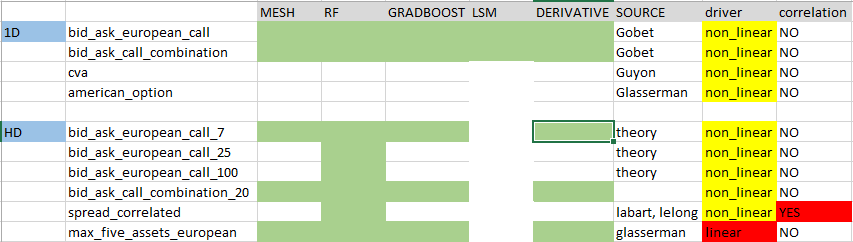
\includegraphics[scale=0.5]{overview.png}
	
\end{frame}

 \begin{frame}
 \frametitle{European Call One Dimension : expected = 7.15}
	
	\centering
	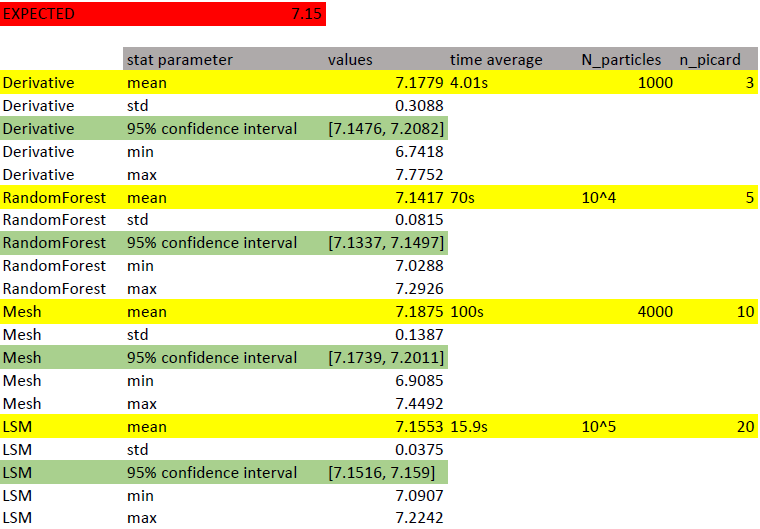
\includegraphics[scale=0.4]{bid_ask_call_1d.png}

 \end{frame}
 
 

 
 
 \begin{frame}
 	\frametitle{Spread Call One Dimension : expected = 2.95 (Gobet)}
 	
 	\centering
 	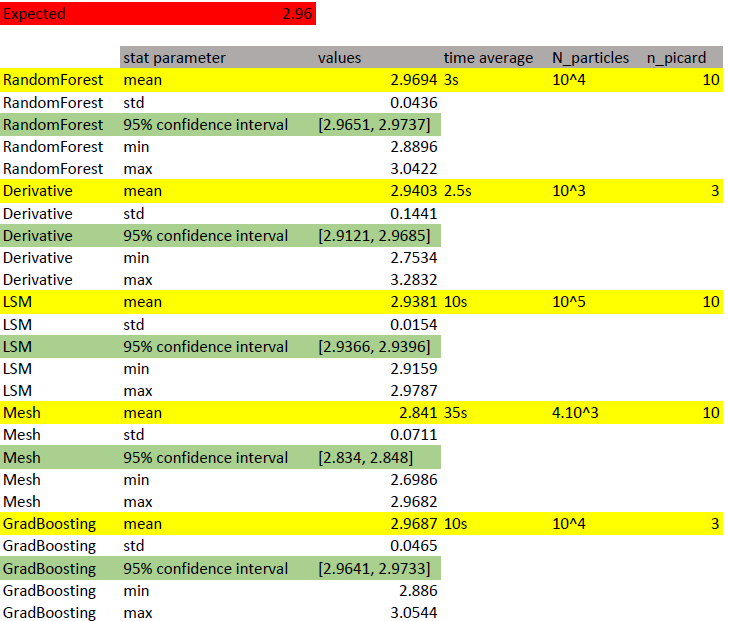
\includegraphics[scale=0.4]{bid_ask_spread_1d_results.png}
 \end{frame}
 
 
\begin{frame}{European bid-ask Basket Option on 7 assets : expected = 3.30 (Black-Scholes)}
	
	
	\centering
	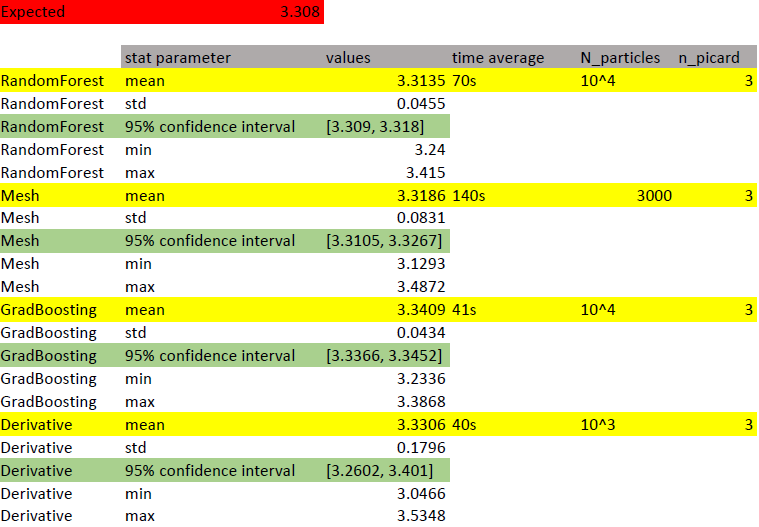
\includegraphics[scale=0.4]{bid_ask_call_7d.png}
	
	
\end{frame}

 \begin{frame}
 	\frametitle{Spread Call on 20 assets : expected = 5.71 (simulation in 1dim)}
 	\centering
 	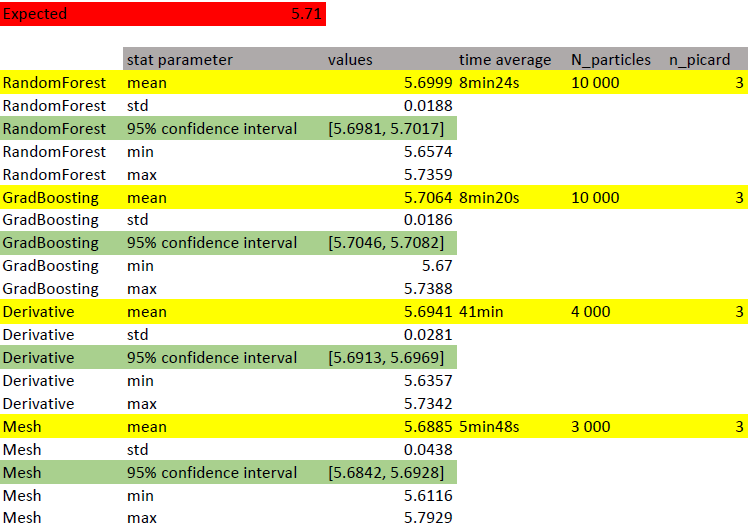
\includegraphics[scale=0.4]{bid_ask_call_combination_20_dim.png}
 \end{frame}

\begin{frame}
	\frametitle{Bid-ask Call on 25 and 100 assets using only RandomForest}
	\centering
	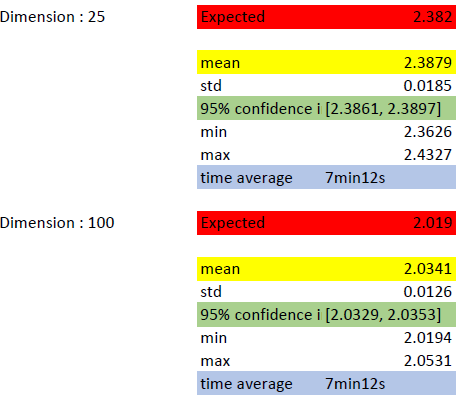
\includegraphics[scale=0.4]{25and100.png}
\end{frame}

\begin{frame}
	\frametitle{Max Call on 5 assets (linear driver)}
	\centering
	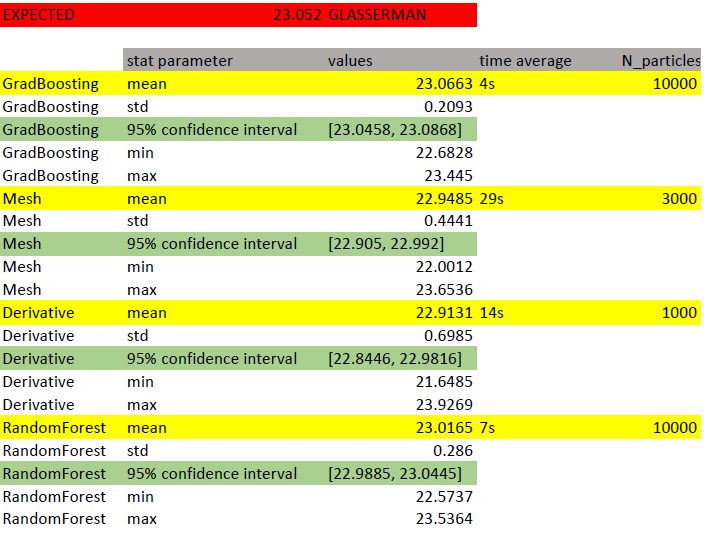
\includegraphics[scale=0.4]{max_call_5d.png}
\end{frame}

\begin{frame}
	\frametitle{Payoff ($(S_1 - S_2)^+$) (linear driver but with Z)}
	\centering
	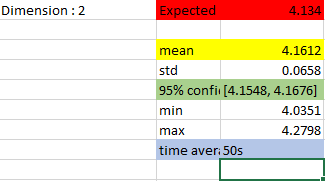
\includegraphics[scale=0.7]{spread_correlated.png}
\end{frame}

\begin{frame}{Remarks}
	\begin{itemize}
		\item The one dimensional examples look good after the calibration of Max\_leaf\_nodes parameter 
		\item The high dimensional examples are quite accurate, but the tree regression is costly in time. 
		\item Thinking about using warm\_start parameter ...
	\end{itemize}
\end{frame}

\section{What's next}

\begin{frame}
	\begin{itemize}
		\item 2-BSDE 
		\item writing
		\item hyperbole implementation maybe ...
	\end{itemize}
\end{frame}
 
\end{document}